\chapter{Sistema de Filtragem}
\label{chap:sistema_filtragem}

Como visto no capítulo \ref{chap:lhc}, um volume enorme de informação é gerado a cada colisão no LHC. Viu-se, também, que os eventos de possível interesse para a detecção do bóson de Higgs, ou dos demais canais físicos de interesse, ocorrem com um período que varia de algumas horas a até dias de operação. Como cada evento, ao interagir com os detectores do ATLAS, produz aproximadamente 1,5 Mbyte de informação, e espera-se uma taxa de 40 MHz de eventos sendo gerados pelo LHC, o fluxo de dados será da ordem de 60 TBytes por segundo \cite{bib:tdaq_tdr}, impossibilitando o armazenamento completo desses eventos para análise \emph{offline}. Desta maneira, um sistema de filtragem \emph{online} \cite{bib:real_time_processing} torna-se indispensável para o experimento. O sistema de filtragem deverá identificar os padrões de decaimento do Higgs, e demais eventos de interesse, para poder localizá-los na massa de eventos com física ordinária, produzida pelas interações mal-sucedidas (interações que produzem canais físicos já conhecidos e que, portanto, significam ruído de fundo para o experimento).

O sistema de filtragem (\emph{trigger}) do ATLAS e o sistema de aquisição de dados é baseado em três níveis sequenciais de seleção \emph{online} de eventos. Partindo de uma taxa de eventos de 40 MHz, a taxa de eventos armazenados precisa ser reduzida, ao final do processo de seleção, para aproximadamente 100 Hz para armazenamento em base de dados e posterior análise \emph{offline}. Enquanto se requer uma alta taxa geral de rejeição, a eficiência na identificação dos eventos de interesse precisa ser elevada, de forma a ser capaz de reter eventos físicos raros \cite{bib:lvl1_trigger_tdr}.

\begin{figure}
\begin{center}
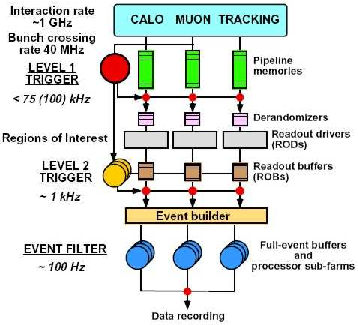
\includegraphics[height = 7.5cm]{block_diagram_trigger}
\caption{Diagrama em blocos do sistema de filtragem.}
\label{fig:block_diagram_trigger}
\end{center}
\end{figure}

Observa-se, na Figura \ref{fig:block_diagram_trigger}, o diagrama em blocos do sistema de \emph{trigger}. Como se percebe, o mesmo está dividido em três níveis principais de validação. A informação gerada pelos detectores é passada para o primeiro nível, que realiza a análise inicial, com granularidade reduzida. Os eventos aprovados pelo primeiro nível são armazenados em \emph{buffers} de leitura, para que possam ser acessados pelos níveis seguintes. O segundo nível opera somente sobre as regiões marcadas pelo primeiro nível, validando a decisão do mesmo, desta vez utilizando a granularidade total dos detectores. Em seguida, os eventos aprovados no segundo nível são enviados ao filtro de eventos (terceiro nível), onde a informação completa de cada evento é utilizada. Por fim, os eventos que são aprovados pelo filtro de eventos são enviados para armazenamento em disco para posterior análise \emph{offline}. Maiores detalhes sobre os três níveis de filtragem serão apresentados a seguir.


\section{Primeiro Nível de \emph{Trigger}}

O primeiro nível de \emph{trigger} (LVL1) realiza a seleção inicial, baseando-se na informação obtida com granularidade reduzida (baixa resolução) gerada por um sub-conjunto de detectores (calorímetros e câmara de múons). A granularidade neste nível é reduzida, uma vez que o tempo para a tomada de decisão neste nível é tão curto que torna-se necessário a redução da quantidade de informação a ser processada, para aumentar a velocidade de processamento. A redução da granularidade é produzida através do agrupamento das células dos calorímetros em conjuntos contendo 6 células, onde as céluas de cada conjunto são analogicamente somadas, produzindo um único sinal. Consequentemente,  este nível só descarta eventos com características bem distintas dos canais de interesse desejados. Múons de momento transverso ($P_T$) elevado são identificados usando apenas as chamadas câmaras de \emph{trigger}, câmaras de placas resistivas no barril, e câmaras de abertura fina nas beiradas \cite{bib:muon_spectrometer_tdr}. A seleção do calorímetro é baseada na informação com granularidade reduzida obtida dos calorímetros do eletromagnético e hadrônico \cite{bib:tdr_liquid_argon, bib:tile_calorimeter_tdr}.


Conforme discutido em \cite{bib:atlas_trigger_status_report}, a maioria das análises físicas que foram consideradas no ATLAS podem ser feitas, no primeiro nível, usando critérios de seleção relativamente simples. Entretanto, a implementação do primeiro nível é flexível e pode ser programada para selecionar eventos usando critérios mais elaborados.

\begin{table}
\centering
\footnotesize
\begin{tabular}{|l|c|}
\hline
\textbf{Evento de Interesse} & \textbf{Freqüência (kHz)}\\
\hline
Múon, $p_T$ $>$ 20 GeV & 4 \\
\hline
Par de múons, $p_T$ $>$ 6 GeV & 1 \\
\hline
Grupo único EM (eletromagnético) isolado, $E_T$ $>$ 30 GeV & 22 \\
\hline
Par de grupos EM isolados, $E_T$ (energia transversa) $>$ 20 GeV & 5 \\
\hline
Jato, $E_T$ $>$ 290 GeV & 0.2 \\
\hline
Três jatos, $E_T$ $>$ 130 GeV & 0.2 \\
\hline
Quatro jatos, $E_T$ $>$ 90 GeV & 0.2 \\
\hline
Jato, $E_T$ $>$ 100 GeV e perdendo $E_T$ (\emph{missing energy}) $>$ 100 GeV & 0.5 \\
\hline
Tau, $E_T$ $>$ 60 GeV e perdendo $E_T$ $>$ 60 GeV & 1 \\
\hline
Múon, $p_T$ $>$ 10 GeV e grupo EM isolado, $E_T$ $>$ 15 GeV & 0.4 \\
\hline
Outros eventos & 5 \\
\hline
\textbf{Total} & $\sim$40\\
\hline
\end{tabular}
\normalsize
\caption{Exemplo de freqüência de observação de eventos no primeiro nível, com luminosidade máxima ($L = 10^{34}$ cm$^{-2}$
s $^{-1}$)}
\label{tab:frequencia_eventos_lvl1}
\end{table}

A taxa máxima de saída do primeiro nível de filtragem está limitada em 75 kHz (podendo ser expandida para 100 kHz). Conforme pode-se concluir da Tabela \ref{tab:frequencia_eventos_lvl1}, as taxas estimadas dos eventos de interesse correspondem, no total, à metade do limite máximo de aceitabilidade do primeiro nível. Entretanto, devido a incertezas intrínsecas nos cálculos, esta margem de segurança não está superestimada \cite{bib:lvl1_trigger_tdr}.

Um requerimento básico para o primeiro nível é que este deve identificar unicamente colisões de interesse. Dado o pequeno (25 ns) intervalo de tempo entre choques de dois pacotes de prótons, esta é uma consideração não trivial. No caso dos calorímetros, por exemplo, um desafio considerável a ser vencido é que o formato do pulso gerado por estes dispositivos pode se estender por várias colisões (efeito de \emph{pile-up} \cite{bib:knoll_radiation_detection}).

É importante que se mantenha o tempo de latência (tempo para formar e distribuir a decisão do filtro) no valor mais baixo possível. Durante este tempo, a informação de todos os canais do detector precisa ser retida em memórias do tipo \emph{pipeline}. Estas memórias estão geralmente contidas em circuitos integrados, posicionadas próximas ou junto ao detector, freqüentemente em regiões inacessíveis e imersas em ambientes de forte radiação. A latência do primeiro nível, medida do instante de uma colisão próton-próton até a decisão do primeiro nível estar disponível para o nível seguinte, deve ser menor que 2,5 $\mu$s. De forma a atingir esta exigência, o primeiro nível de \emph{trigger} está sendo implementado em \emph{hardware} de baixa programabilidade do tipo FPGAs (\emph{Field Programmable Gate Array}) \cite{bib:fpga}, devido à sua velocidade. O tempo de latência desejado para este nível de \emph{trigger} foi, então, estipulado para 2 $\mu$s, deixando 500 ns de margem de segurança \cite{bib:lvl1_trigger_tdr}.

Os eventos selecionados recebem uma etiqueta do LVL1 com a identificação do canal físico ao qual pertencem, e em seguida são lidos dos \emph{drivers} de saída dos detectores (\emph{Read Out Drivers} - ROD) e propagados para os \emph{Readout Buffers} (ROB) através dos cabos de leitura (\emph{Read Out Links} - ROL), ficando, assim, disponíveis como fragmentos de informação (vide Seção~\ref{sec:eformat}) para o sistema de filtragem de alto nível.\footnote{A parte de alto nível do sistema de \emph{trigger} corresponde ao segundo e terceiro nível, visto que são desenvolvidos em \emph{software} e executados em computadores de uso geral.}. Entretanto, de forma a reduzir o volume de tráfego de dados para o segundo nível, e, conseqüentemente, aumentar a banda passante entre estes dois níveis, o primeiro nível já marca as regiões de interesse (\emph{Region of Interest} - RoI), que correspondem a regiões do detector onde houve a incidência de algum evento, e que foi aceito pelo primeiro nível, de tal maneira que o segundo nível observará somente estas regiões de interesse, e não toda a área do detector.




\section{O Sistema de Filtragem de Alto Nível}
\label{sec:htl}

\begin{figure}
\begin{center}
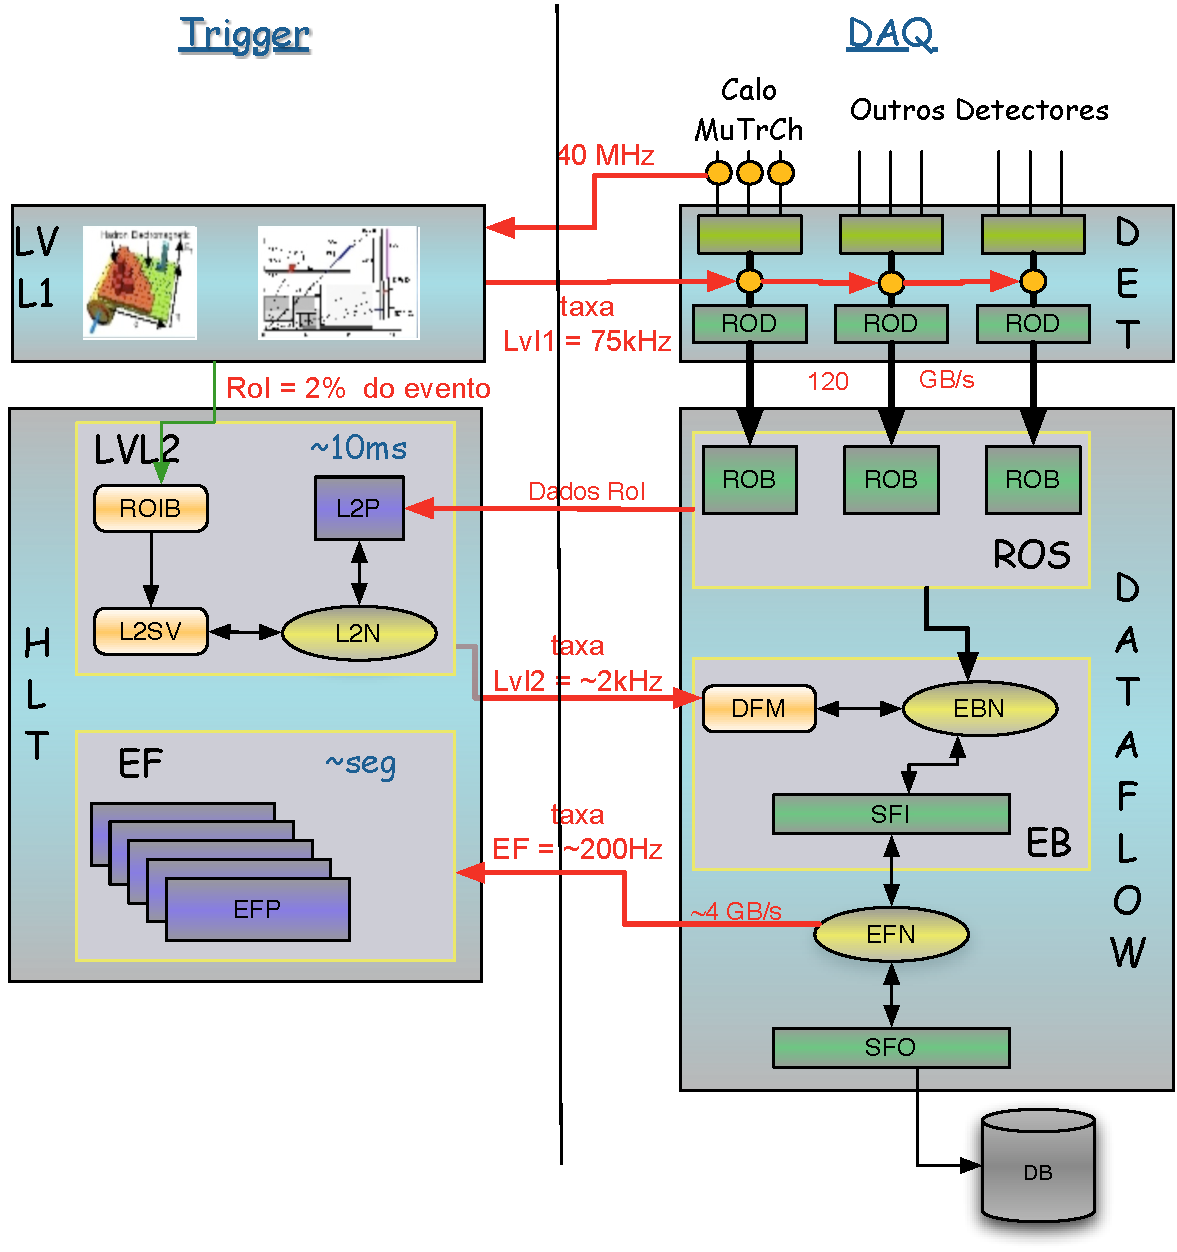
\includegraphics[height = 10cm]{tdaq_diagram}
\caption{Diagrama detalhado em blocos do sistema de filtragem de alto nível.}
\label{fig:tdaq_diagram}
\end{center}
\end{figure}

O sistema de filtragem de alto nível do ATLAS (\emph{High Level Trigger} - HLT) é composto pelo segundo nível \emph{LVL2} e pelo filtro de eventos (\emph{Event Filter - EF}), por serem todos implementados em \emph{software} com linguagem de programação de alto nível. A Figura~\ref{fig:tdaq_diagram} apresenta os detalhes desta parte do sistema de filtragem. Após a filtragem do LVL1, os eventos aprovados ficam disponíveis na forma de fragmentos nos sistemas de leitura (\emph{Read-Out Systems - ROS}). Além disso, a informação à respeito das RoIs etiquetadas pelo LVL1 são enviadas para o  construtor de RoI (\emph{RoI Builder} - RoIB). Este agrupa os fragmentos de informação gerados pelos diferentes detectores do ATLAS, e transmite o registro gerado por este agrupamento para um supervisor do segundo nível (\emph{LVL2 Supervisor - L2SV}) que ficará responsável por atribuir a uma unidade de processamento do segundo nível  (\emph{LVL2 Processing Unit} - L2PU) a RoI recebida. A L2PU então valida a etiqueta do LVL1, usando a granularidade total dos detectores, e retorna o resultado para o L2SV. Este envia o resultado para o gerenciador de fluxo de dados (\emph{Dataflow Manager - DFM}), para que o evento seja apagado em caso de rejeição, ou propagado para o filltro de eventos, caso sejam aprovados.  O DFM seleciona um dos processadores da fazenda de entrada (\emph{Sub-Farm Intut - SFI}) para que o mesmo solicite aos ROS toda a informação disponível do evento em questão. Uma vez a informação disponível, o SFI seleciona um dos processadores do filtro de eventos (\emph{EF Processor - EFP}), para que o mesmo realize analises detalhadas, usando toda a informação disponível para cada evento, e gerando, assim, a decisão final do sistema de filtragem. Os eventos finalmente aprovados são enviados às fazendas de saída (\emph{Sub-Farm Outtut - SFO}) para que possam ser armazenados em mídia permanente, para posterior análise \emph{offline}. A Tab.~\ref{tab:hlt_comp} apresenta o número de processadores necessários para cada módulo do sistema de filtragem de alto nível do ATLAS, considerando máquinas com 4 núcleos de processamento com \emph{clock} de 3 GHz cada.

Todo o segundo nível de filtragem foi desenvolvido utilizando, o máximo possível, tecnologias padronizadas (comerciais) \cite{bib:paper_lvl2}, visando fácil reposição de material e implementação simplificada. Todos os processadores são de uso geral (tipo PC) e praticamente todas as comunicações entre estes dispositivos são feitas através de \emph{switchs} Gigabit Ethernet, devido à velocidade, confiabilidade e padronização do protocolo. Todas as aplicações também estão desenvolvidas utilizando técnicas de orientação a objetos e implementadas em C++ \cite{bib:herbert_schildt_c++}.

\begin{table}
\begin{center}
\begin{tabular}{|l|c|}
\hline
Módulo & N$^o$ Processadores \\
\hline
ROS & 225 \\
\hline 
RoIB & 1 \\
\hline 
L2SV & 50 \\
\hline 
L2PU & 500 \\
\hline 
DFM & 1 \\
\hline 
SFI & 120 \\
\hline 
EFP & 1600 \\
\hline 
SFO & 35 \\
\hline 
Controle & 90 \\
\hline
\end{tabular}
\end{center}
\caption{Quantidade de processadores necessários para cada módulo do sistema de filtragem de alto nível do ATLAS.}
\label{tab:hlt_comp}
\end{table}

O sistema de filtragem de alto nível está dividido em duas partes: a aquisição e controle de dados e a parte de processamento dos eventos produzidos pelo ATLAS. Ambas descritas a seguir.

\subsection{Aquisição e Controle de Dados (\emph{Data Aquisition and Control - DAQ})}
\label{sec:daq} 

O DAQ é responsável pela propagação dos eventos pelo sistema de filtragem de alto nível do ATLAS. É responsabilidade de seus módulos garantir a integridade e correto fluxo da informação por todo o sistema. Além disso, o DAQ precisa assegurar que a informação chegará em tempo hábil, para atender os restritos requisitos de tempo. Por fim, o DAQ também é responsável por prover mecanismos de monitoração dos seus módulos, de forma a assegurar que os mesmos estejam funcionando corretamente. A seguir, serão apresentados os módulos que compõem o DAQ. 

\subsubsection{Sistemas de Leitura (\emph{Read-Out Systems - ROS})}
\label{sec:ros}

Os ROS são computadores de uso geral, tipo PC, que servem de interface entre o sistema de filtragem de alto nível e os eventos aprovados pelo LVL1. O ROS possui 3 componentes rincipais: o \emph{Buffer} de Leitura (\emph{Read-Out Buffer} - ROB), o \emph{IOManager} e o \emph{Controlador Local} .

O ROB provê armazenamento temporário dos fragmentos de informação produzidos por um dado ROD, para que sejam acessados pelo LVL2 e pelo Construtor de Eventos. Consequentemente, o ROB receberá fragmentos na taxa do LVL1, ou seja, 100 kHz. Todos os fragmentos de informação vindo de um ROD ficam armazenados pelo tempo de latência do LVL2, e aproximadamente 3\% destes, durante o tempo da construção do evento pelo Construtor de Eventos. Cada ROS possui 12 ROB, e cada ROB fica conectado a um único ROD através de um ROL. Para o tráfego dos fragmentos de informação com o sistema de filtragem, é utilizado uma rede gigabit ethernet dedicada para os dados do LVL2, e outra para os dados do Construtor de Eventos, de forma a diminuir o tempo de espera por fragmentos de informação. 

O \emph{IOManager} processa os requisitos de dados oriundos das L2PU e dos SFI. De acordo com o critério especificado na requisição do dado, o \emph{IOManager} coleta um ou mais fragmentos de ROB de um ou mais ROB, gera um fragmento de ROS (vide Seção~\ref{sec:eformat}) contendo os fragmentos de ROB selecionados, e envia este fragmento para o componente solicitante. O \emph{IOManager} também recebe do DFM requisições para liberar o espaço utilizado por fragmentos de ROB que já foram utilizados e devem ser apagados. Para otimizar a performance global do ROS, o \emph{IOManager} permite transmissões simultâneas de dados, isto é possível graças à arquitetura \emph{multi-thread} adotada no design deste componente.

 O Controlador Local prôve a interface entre o ROS e o software \emph{online}. Ele configura, controla e monitora todos os componentes dentro do ROS. A monitoração compreende tanto a monitoração operacional (tamanho de filas, páginas de memória utilizada, etc), e a provisão de amostras dos fragmentos de informação fluindo pelo ROS, com o objetivo de monitorar os detectores. O Controlador Local comunica-se com o software \emph{online} através da rede de controle, de tal forma a não impactar na velocidade de transmissão de fragmentos de informação do ROS.


\subsubsection{Geradores de Regiões de Interesse (\emph{RoI Builders - RoIB})}
\label{sec:roib}

Para cada evento aceito, o primeiro nível envia informações como a posição da RoI e valores de limiar alcançados. O RoIB combina estes fragmentos em um único registro que é passado a um L2SV. No esquema básico, cada L2SV verá apenas um subconjunto de L2P, de tal forma que a escolha do L2SV afeta o balanço de carga entre os L2P. O critério de seleção de L2SV utilizado pelo RoIB é o \emph{round-robin} \cite{bib:modern_operating_systems}.


\subsubsection{Supervisor do Segundo Nível (\emph{LVL2 Supervisor - L2SV})}
\label{sec:l2sv}

Os supervisores do segundo nível (L2SV) são um pequeno grupo de 50 processadores que supervisionam o fluxo de eventos no segundo nível e atuam como mediadores entre os sistemas do primeiro e do segundo nível. De forma a simplificar o gerenciamento dos processadores, os processadores utilizados para este fim serão de tipo similar aos que serão utilizados para a seleção de eventos. Entretanto, cada processador supervisor precisa de uma interface para receber dados do RoIB \cite{bib:tdaq_tdr}.

\begin{figure}
\begin{center}
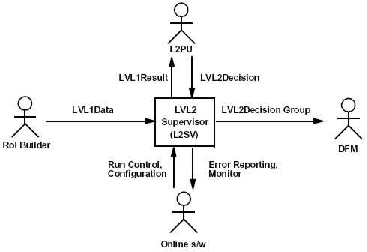
\includegraphics[height = 6cm]{lvl2_supervisor}
\caption{Contexto do supervisor do segundo nível.}
\label{fig:l2sv}
\end{center}
\end{figure}

O contexto do supervisor do L2SV é indicado na Figura \ref{fig:l2sv}. O L2SV recebe do RoIB a informação do primeiro nível em um único registro. O supervisor seleciona, então, um L2P para o evento e passa para uma das unidades de processamento (L2PU)\footnote{Um L2P pode ter várias L2PUs sendo executadas simultaneamente, visando maximizar a eficiência de uso da CPU.} o dado do primeiro nível. Uma vez que o algoritmo foi executado e uma decisão quanto ao evento foi tomada, a mensagem de decisão é passada para o L2SV. O Resultado é propagado, então, para o controlador de fluxo de dados (\emph{Data Flow Manager} - DFM) e para o L2HR. 

Ao selecionar um L2P, o supervisor o faz através de uma função de balanceamento de carga, examinando o numero de eventos na fila e associe cada evento ao processador menos carregado \cite{bib:tdaq_tdr}.


\subsubsection{Processadores do Segundo Nível (\emph{LVL2 Processors} - L2P)}
\label{sec:l2p}

O algoritmo de seleção do segundo nível é executado em uma rede de processadores do tipo PC com múltiplos núcleos de processamento. O tempo total de decisão médio, para cada evento do segundo nível, é de aproximadamente 10 ms. Entretanto, haverá uma larga variação entre os tempos gastos com cada evento, uma vez que certos eventos podem ser descartados logo no início do processo de seleção do segundo nível, enquanto que outros terão que ser propagados até o fim, para que uma decisão possa ser tomada. Cada evento será manipulado por um único processador, que requisitará dados aos ROS de cada RoI somente quando solicitado pelo algoritmo. Para manter uma alta eficiência de utilização de cada processador, enquanto este espera por um evento, vários eventos estarão sendo processados em paralelo dentro de um mesmo processador, tanto através da execução de várias cópias do \emph{software} de seleção, bem como pelo uso de múltiplas \emph{threads} dentro de um mesmo programa.

O processamento é executado em um único aplicativo rodando em cada processador. Este aplicativo contém três componente principais: a unidade de processamento do segundo nível (\emph{LVL2 Processing Unit} - L2PU), a interface de comunicação PESA (\emph{PESA Steering Controller} - PSC) e o \emph{software} de seleção de eventos (\emph{Events Selection Software} - ESS). A L2PU lida com o fluxo de dados com outras partes do sistema de \emph{trigger}, incluindo envio de mensagens, configuração, controle e supervisionamento. A PSC é executada dentro da L2PU e provê o ambiente e serviços necessários para o ESS. Como a L2PU controla a comunicação com o L2SV e os ROS, algumas interfaces precisam ser providas para as várias mensagens entre a L2PU e o ESS. A PSC provê a interface para o resultado do primeiro nível e retorna o resultado do segundo nível. Maiores detalhes sobre o ESS estão apresentados na Seção \ref{sec:offline}.

O desenvolvimento e implementação das L2PUs são baseados em um ambiente \cite{bib:tdaq_tdr} do qual são utilizados os seguintes serviços: controle, inicialização e configuração de aplicativos, relatório de erros, monitoração e envio de mensagens de aplicativos e instrumentação (este último para avaliação de performance).

As L2PU se comunicam com os supervisores do segundo nível, dos quais a mesma recebe a informação da RoI (gerada pelo primeiro nível) e para os quais ela retorna a decisão do segundo nível. Os dados da RoI (provenientes de vários ROB) são requisitados dos ROS, de acordo com a necessidade dos algoritmos de seleção.

Os algoritmos de seleção propriamente ditos são executados dentro de uma das \emph{threads} de execução (\emph{Worker Threads}), cada uma processando um evento. Esta abordagem \emph{multi-thread} foi adotada para evitar a parada da CPU enquanto a mesma aguarda pelo dado solicitado ao ROS. Este recurso também permite o uso eficiente de processadores contendo múltiplas CPUs, mas requer que o algoritmo de seleção de eventos seja seguro, no que diz respeito a esta implementação. Alguns serviços assíncronos (monitoração de aplicativos, entrada de dados) também são executados em \emph{threads} separadas.

\begin{figure}
\begin{center}
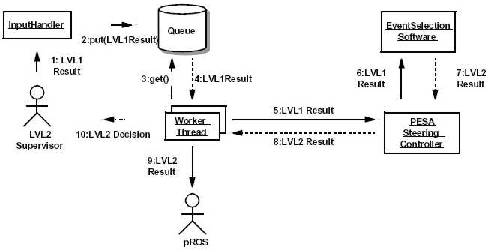
\includegraphics[height = 6cm]{eventsflow_lvl1_to_lvl2}
\caption{Fluxo de eventos aplicados a cada evento recebido do primeiro nível e que leva à decisão do segundo nível.}
\label{fig:app_l2p}
\end{center}
\end{figure}

Pode-se observar, na Figura \ref{fig:app_l2p}, o que acontece para cada evento no LVL2. O supervisor do segundo nível seleciona uma L2PU e envia o resultado do primeiro nível. Esta L2PU armazena o resultado recebido em uma fila compartilhada. Quando uma \emph{thread} fica disponível, a mesma retira da fila um evento, inicia o processamento do mesmo e produz, ao final, o resultado do segundo nível. Finalmente, a decisão do segundo nível é gerada a partir do resultado gerado pela \emph{thread} e retornado ao supervisor do segundo nível. Se o resultado for positivo, o resultado é enviado, também, para o L2RH.


Quando os algoritmos de seleção necessitam de dados dos ROBs, o fornecedor de dados do ROB é ativado e seu funcionamento pode ser observado na Figura \ref{fig:l2pu_dc}. O coletor de dados dos ROB cuida das requisições de envio para os ROS apropriados, espera até que todos os dados cheguem, monta os fragmentos de ROS recebidos em uma lista de fragmentos de ROB que são retornados ao chamador. Em \cite{bib:tdaq_tdr}, exames de performance relacionados à coleta de dados de RoIs pelos ROB foram executados e os resultados excederam, por uma larga margem, as especificações de I/O exigidas pelo projeto.

\begin{figure}
\begin{center}
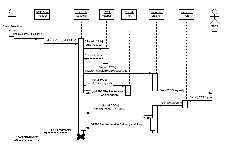
\includegraphics[width = 12cm]{l2pu_data_collection}
\caption{Coleta de dados dentro da lista de ROB (correspondentes a uma RoI) pela L2PU.}
\label{fig:l2pu_dc}
\end{center}
\end{figure}

Outro componente de destaque do L2P é a PSC. A PSC é o componente do sistema de \emph{trigger} de alto nível que realiza a interface entre a L2PU e o ESS. Os objetivos da PSC são três:

\begin{enumerate}

\item Permitir que a L2PU hospede e controle \emph{softwares} de seleção desenvolvidos \emph{offline}.

\item Permitir que os softwares de orientação possam ser compartilhados com o terceiro nível.

\item Prover um mecanismo para transmitir os resultados dos níveis 1 e 2 entre o sistema de fluxo de dados e o ESS.

\end{enumerate}

A chave do desenvolvimento da PSC é colocar esta interface onde a funcionalidade do fluxo de dados do segundo nível e o ESS podem ser perfeitamente separados. O local escolhido foi a máquina de estados finita da L2PU. A PSC provê os meios necessários para encaminhar mudanças no estado de controle de execução do software de fluxo de dados do segundo nível para o ESS, visto que o ESS está sendo desenvolvido no sistema \emph{offline} Athena (vide seção \ref{sec:offline}).


É apresentada, na Figura \ref{fig:l2pu_pesa}, a seqüência de interações da PSC entre a L2PU e o ESS. Na figura, pode-se observar três estados: 

\begin{enumerate}

\item \textbf{Configuração}: durante a fase de configuração, dados sobre condições e configurações são obtidos de uma base de dados externa, via interface \emph{online} do sistema de \emph{trigger}. Estes dados são, então, usados para configurar o ESS e todos os componentes associados.

\item \textbf{Início}: após o início, a PSC recebe uma diretiva de evento de execução, com um resultado do primeiro nível como argumento. A PSC, então, retorna (após execução do ESS) o resultado do segundo nível, direto à L2PU.

Um importante aspecto desta abordagem é que o manuseio de eventos do segundo nível é gerenciado inteiramente pelo pacote de coleta de dados. A PSC não precisa interagir diretamente com a \emph{thread} de entrada, o L2SV ou com o L2RH. As requisições por fragmentos de dados são ocultas, uma vez que são realizadas pelo serviço provedor de dados.

\item \textbf{Parada}: após a parada, a PSC termina a execução de algoritmos. Neste estágio, relatórios de execução podem ser produzidos para o processo de seleção.

\end{enumerate}


\begin{figure}
\begin{center}
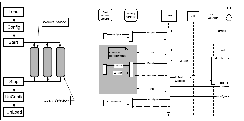
\includegraphics[height = 7.5cm]{l2pu_and_pesa_steering_controller}
\caption{A máquina de estados finita da L2PU (esquerda) e a interface PESA (direita).}
\label{fig:l2pu_pesa}
\end{center}
\end{figure}

\begin{figure}
\begin{center}
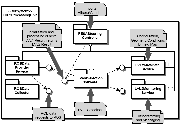
\includegraphics[height = 6cm]{dependencies_ess}
\caption{Dependências do ESS executando a seleção de eventos na L2PU.}
\label{fig:dependencies_ess}
\end{center}
\end{figure}

Pode-se observar, na Figura \ref{fig:dependencies_ess}, o diagrama para a execução do ESS na L2PU. A comunicação com sistemas externos e sub-sistemas, incluindo o L2SV e o ROS, estão ocultos do ESS. O ESS é inicializado conforme a Figura \ref{fig:l2pu_pesa}. O PSC fornece ao ESS os resultados do primeiro nível e requisita a seleção do segundo nível. Para fornecer o resultado do segundo nível, o ESS precisa acessar o serviço de fornecimento de dados do ROB. A requisição de dados ao ROB é enviada através do serviço de fornecimento de dados do ROB para o coletor de dados do ROB.


\subsubsection{Manipulador de Resultados do Segundo Nível (\emph{LVL2 Result Handler} - L2RH)}

Para todos os eventos aceitos pelo segundo nível, os detalhes do processamento deste nível (e o resultado completo do primeiro nível, recebido pelo supervisor) são fornecidos pela L2PU para que sejam incluídos ao evento. Entretanto, os ROS só armazenam dados provenientes do LVL1. Para resolver este problema, o L2RH foi desenvolvido. Este componente opera de maneira bastante similar ao ROS, só que recebe a informação gerada pelo LVL2. A informação do LVL2 é enviada via rede como um fragmento de ROB para o L2RH, onde é armazenada, enquanto aguarda sua requisição pelo construtor de eventos, que enxerga o L2RH como um ROS. Quando o evento é construído, o L2RH é inserido com todos os outros ROSs, de forma a incluir o resultado do segundo nível na construção do evento, que será enviado ao filtro de eventos. Uma única unidade como essa é suficiente para lidar com o volume de dados ao final do segundo nível, onde se espera um fluxo de uns poucos kilobytes por segundo, considerando uma taxa de aceitação de 3 kHz.


\subsubsection{Gerenciador de Fluxo de Dados (\emph{Dataflow Manager} - DFM)}

Este componente se encarrega de receber os resultados das decisões realizadas pelo LVL2. Eventos rejeitados são salvos em uma fila, de forma que, quando esta fila enche, o DFM dispara uma mensagem para todos os ROS solicitando que estes removam de seus ROB os fragmentos de informação pertencentes aos eventos rejeitados. Para os eventos aprovados, o DFM opera de maneira análoga ao L2SV. Ele seleciona um SFI menos carregado e envia a este as informações de um dado evento aprovado, para que este seja construído pelo SFI. Ao final da construção do evento, o DFM solicita aos ROS que apaguem os fragmentos de informações referentes a este evento, visto que durante a construção, estes fragmentos são copiados para o SFI, de forma a liberar espaço nos ROB. 


\subsubsection{Fazendas de Entrada (\emph{Subfarm Input} - SFI)}

O SFI é o dispositivo encarregado de requisitar e receber todos os fragmentos de dados de um determinado evento, para a que o mesmo seja montado e propagado ao filtro de eventos. Após a montagem do evento, o SFI informa ao DFM que o evento já foi corretamente montado, de forma que o DFM possa solicitar aos ROS que apaguem as informações referentes ao evento montado. Para aumentar a eficiência de utilização de um SFI, várias \emph{threads} operam concorrentemente, permitindo a construção de vários eventos em paralelo dentro de um mesmo SFI. O SFI também é responsável por enviar a um processador do filtro de eventos o evento totalmente construído. Somente após o processador do filtro de eventos acusar o correto recebimento do evento montado, o mesmo é apagado da memória do SFI \cite{bib:eb}.


\subsubsection{Processador do Filtro de Eventos (\emph{Event Filter Processors} - EFP)}

O EFP é o componente que solicitará ao SFI ao qual está conectado, um evento construído, para realizar a validação final sobre o mesmo. Cada EFP executa um programa de controle de fluxo de dados (\emph{Event Filter Dataflow} - EFD) que receberá dos SFI os eventos construídos. Adicionalmente, cada EFP possui várias Unidades de Processamento (\emph{Processing Tasks} - PT). As PT são encarregadas de processar os eventos recebidos pelo EFD. Enquanto a L2PU observa apenas parte do detector (RoI), a PT analisará toda a informação disponível para cada evento.  Quando uma dada PT completa o processamento de um evento, ela requisita um novo. Os dados gerados pela PT durante o processamento são anexados ao evento completo, caso tenha sido aceito pela PT. Os eventos aceitos são classificados e movidos para o respectivo SFO, para serem gravados em arquivos em disco.

Os EFP estão organizados em conjuntos, onde cada conjunto está associado a um ou mais SFI ou SFO. SFI, SFO e os EFP estão conectados através de um \emph{switch} Ethernet de alta velocidade (Gigabit Ethernet).


\subsubsection{Fazendas de Saída (\emph{Subfarm Output} - SFO)}

Após a validação final de cada evento pelas PT, os eventos aprovados devem ser finalmente  armazenados em mídia permanente para posterior análise \emph{offline}. Quando um EFD aprova um evento, ele o envia para o SFO, para que o mesmo o armazene em arquivos em disco. Estes arquivos são posteriormente acessados por um sistema de armazenamento em massa para armazenamento definitivo \cite{bib:tdaq_tdr}.


\subsubsection{Comunicação entre os Módulos do Sistema de Filtragem}

Para o transmissão de dados entre os módulos do sistema de filtragem de alto nível do ATLAS, utiliza-se \emph{switchs} Gigabit \emph{ethernet}. Para lidar com o enorme fluxo de informações, existem redes específicas para cada parte do sistema de filtragem de alto nível. A rede de controle (\emph{Control Network} - CTRLN) conecta todos os dispositivos. Informações de configuração, monitoração, notificações de erros são transmitidas por cada módulo utilizando esta rede. A rede de tráfego do segundo nível (\emph{LVL2 Network} - L2N) é responsável pelo tráfego de dados dos componentes pertencentes a este nível. Os L2SV enviam as informações sobre a RoI a ser validada para o L2P utilizando esta rede, e as L2PU requisitam aos ROS os fragmentos de informação necessários também utilizando esta rede. A L2N também conecta o L2SV com o DFM e o L2RH. A rede do contrutor de eventos (\emph{Event Bulder Network} - EBN) será utilizada para trafegar os dados a serem construídos entre os ROS, L2RH, DFM e SFI. Por fim, a rede do filtro de eventos (\emph{Event Filter Network} - EFN) conecta os EFP com os SFI e SFO. É apresentado na Figura~\ref{fig:net_design} o diagrama com a conexão das redes de tráfego de dados do sistema de filtragem de alto nível, para melhor visualização.

\begin{figure}
\begin{center}
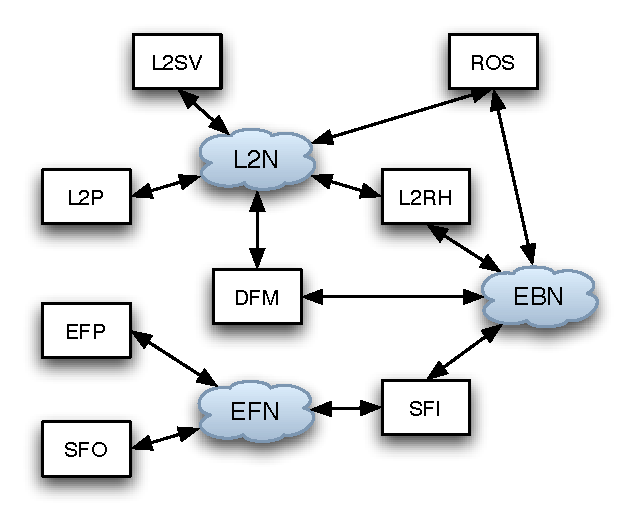
\includegraphics[height = 7cm]{hlt_network_design}
\caption{Diagrama de conexão das redes de dados do HLT.}
\label{fig:net_design}
\end{center}
\end{figure}


Como apresentado nesta seção, o volume de informação trafegando entre o LVL1 e o HLT é muito elevado. Além disso, o LVL1 opera próximo ao ATLAS, enquanto o HLT opera na superfície, separado do LVL1 por aproximadamente 200 metros. Consequentemente, a interface entre estas duas partes possuem alguns requisitos especiais, a saber:

\begin{itemize}

\item Palavra de 32 bits à 40,08 MHz ($\sim160$ Mbyte/s).

\item Resistência à radiação.

\item Latência muito pequena.

\item Comprimento máximo de 300 metros.

\end{itemize}

Estes requisitos tornam inviável a utilização de redes Gigabit \emph{ethernet}. Desta forma, os ROS e o RoIB estão conectados aos detectores do ATLAS por cabos de fibra óptica, usando protocolo de comunicação S-LINK \cite{bib:slink_spec}. O protocolo S-LINK é uma protocolo de comunicação ponto-a-ponto desenvolvido especialmente para atender os rígidos requisitos de transmissão entre o LVL1 e o HLT. Ao contrário de outros padrões, que definem a camada física de transmissão, o S-LINK define uma simples interface FIFO síncrona na qual os sinais de transmissão ficam independentes do canal físico. O mapeamento entre os sinais da S-LINK e do protocolo usado na camada física fica a critério do desenvolvedor do canal de transmissão, de forma que este pode realizar este mapeamento da forma mais adequada à tecnologia adotada no canal de transmissão.


\subsection{Athena}
\label{sec:offline}

O requisito básico exigido pelos físicos para realizarem suas tarefas é um conjunto de programas para realizar simulações de eventos, reconstruções, visualizações, etc. Além de um conjunto de ferramentas que permitam a escrita de programas de análises. Adicionalmente, os físicos desejam algo fácil de usar e extremamente flexível. Por fim, os físicos do ATLAS desejam desenvolver algoritmos de seleção de eventos para operarem \emph{online} no sistema de filtragem do ATLAS.

Para suprir estes requisitos, o Athena foi desenvolvido. O Athena é um \emph{framework} de controle que representa uma implementação concreta de uma arquitetura. A arquitetura por baixo do Athena é a arquitetura do Gaudi \cite{bib:gaudi}, originalmente desenvolvida para o LHCb. Esta arquitetura foi extendida através da colaboração com o ATLAS, e uma arquitetura base, desacoplada a um experimento específico, e também chamada Gaudi foi desenvolvida. O Athena é, então, a união desta arquitetura base com melhorias expecíficas ao ATLAS \cite{bib:athena_dev_guide}. 

O objetivo principal do Athena é isolar seus usuários de detalhes irrelevantes, como que tipo de biblioteca usar para transferência de dados, ou para gerar um gráfico. Para tal, sua arquitetura consiste na especificação de um número de componentes e suas interações entre si. Um componente é um bloco de código que possui uma funcionalidade e interface bem definida. Uma interface é uma coleção de métodos junto com uma descrição sobre o que cada método faz, ou seja, sua funcionalidade. Os principais benefícios desta abordagem são:

\begin{itemize}

\item \textbf{Flexibilidade}: esta abordagem provê simplicidade, dado que componentes podem ser conectados de diferentes maneiras para desempenhar diferentes tarefas.

\item \textbf{Simplicidade}: softwares para acessar, por exemplo, uma base de dados, são normalmente complexos de se aprender. Entretanto, a maioria dos detalhes são de pouco interesse para alguem que deseja simplesmente ler dados e salvar seus resultados. Desta forma, um componente para acessar dados pode ser desenvolvido de forma a fornecer somente a funcionalidade desejada. Além disso, a interface para este componente continuaria a mesma, independentemente da tecnologia de armazenamento utilizada pela base de dados do exemplo em questão. 

\item \textbf{Robustez}: como dito acima, um determinado componente pode ocultar de seu usuário a tecnologia que utiliza. Além de oferecer simplicidade, a vantagem que isto representa é que a tecnologia pode ser alterada sem que o usuário precise sequer saber desta mudança.

\end{itemize}


Alguns dos principais serviços e interfaces do Athena são:

\begin{itemize}

\item \textbf{Pythia}: o Athena provê interface para o Pythia. Este módulo é responsável por simular a colisão de feixes de partículas. 

\item \textbf{Geant}: o Geant é um conjunto de ferramentas que permitem simular a interação de partículas com a matéria. Desta forma, torna-se possível simular o comportamento dos detectores do ATLAS quando excitados por partículas. As simulações de Monte Carlo utilizadas para a análise e desenvolvimento de algoritmos de seleção são produzidas através da simulação de colisões geradas pelo Pythia, e a consequente descrição do comportamento dos detectores do ATLAS utilizando o Geant para descrever como estas partículas produzidas pelo Pythia interagem  com o material que compões dos detectores do ATLAS.  

\item \textbf{Storegate}: O Storegate é um amiente que permite a propagação de dados entre pacotes do Athena. Ele funciona como uma área de armazenamento, onde um dado algoritmo pode identificar e salvar informações geradas pelo mesmo no Storegate, de forma que os algoritmos subsequentes possam recuperá-lo, ao fornecer ao Storegate a chave de identificação do dado desejado.

\end{itemize}


Dado a flexibilidade do Athena, este está sendo utilizado para o desenvolvimento de algoritmos de seleção de eventos. Este algorimtos podem acessar as simulações de Monte Carlo que reproduzem a colisão de partículas e a consequente interação destas com os detectores do ATLAS para realizar processos de extração de características e tomadas de decisão. Muitos destes algoritmos  operam somente em modo \emph{offline}. Entretanto, como dito acima, o Athena também será usado na filtragem \emph{online} do ATLAS, de forma que uma famíilia especial de algoritmos foi desenvolvida para atender a este objetivo.

\subsubsection{Estratégia \emph{Online} para a Seleção de Eventos}

Como dito anteriormente, os eventos de interesse para o experimento ATLAS são bastante raros. Desta forma, lida-se com um volume muito maior de informação irrelevante, do que com eventos de interesse. Desta forma, a melhor estratégia de filtragem é rejeitar, o mais rápido possível, eventos considerados como ruído de fundo. A configuração e capacidades do sistema de filtragem de alto nível são dirigidas pela performance física (seleção de eventos e rejeição de ruído) e pela performance do sistema (velocidade de execução, requisitos de dados). O melhor compromisso entre estes fatores tem que ser encontrado de forma a maximizar a performance física. Para rejeitar eventos o mais rápido possível, uma abordagem de filtragem em etapas foi escolhida pelo ATLAS tanto para o LVL2, bem como para o EF. 

Para esta abordagem, um mecanismo de controle foi desenvolvido. Suas principais características são:

\begin{itemize}

\item Manter-se informado sobre quais algoritmos já foram executados para um dado evento, quais informações foram geradas por cada algoritmo e onde estas estão armazenadas. Adicionalmente, ele provê os mecanismos de persistência e propagação  da informação, e provê mecanismos de acesso à informação gerada por cada algoritmo.

\item Formar e manipular o resultado gerado para cada evento.

\item Acessar os resultados do LVL1 e do LVL2, que dará origem aos subsequentes passos de reconstrução.

\end{itemize}

No contexto deste controle, algumas entidades etão presentes:

\begin{itemize}

\item \textbf{Elemento de \emph{Trigger}}: entidade que é ativada por um determinado algoritmo para sinalizar a validação de um corte.  No LVL1, um elemento de \emph{trigger} é uma RoI. Já no sistema de filtragem de alto nível, eles são gerados através de sequências de algoritmos de extração de características e testes de hipótese.

\item \textbf{Assinatura}:  combinação de elementos de \emph{trigger} que podem levar a uma decisão positiva do sistema de filtragem. Os elementos de \emph{trigger} podem ser combinados por lógica booleana \texttt{AND}, \texttt{OR} e \texttt{NOT}. Adicionalmente a multiplicidade de elementos de \emph{trigger} pode ser configurada. Exemplo: uma assinatura  \texttt{e25i} representa um elétron isolado com energia transversa superior a 25 GeV. Já a assinatura \texttt{2e15i} é a assinatura produzida pelo sistema de filtragem quando dois elétrons isolados e com energia superior a 15 GeV são identificados.

\item \textbf{Menu}: consiste em uma série de assinaturas. Se uma ou mais assinaturas são satisfeitas, o evento é disparado.

\item \textbf{Cadeia}: sequência de algoritmos utiizados para ativar uma determinada assinatura.

\item \textbf{Slice}: um \emph{slice}  é a sequência de processamento utilizada para um tipo de partícula (elétron, fótons, múons, etc) e compreende os três níveis de filtragem (LVL1, LVL2 e EF).

\end{itemize}

É apresentado na figura~\ref{fig:athena_trigger_str} a organização do Athena no que tange a filtragem de alto nível do ATLAS. Podemos observar que um \emph{slice} compreende várias assinaturas contidas em um menu, onde cada uma delas é ativada por uma cadeia de algoritmos. Uma sequência pode ser composta por vários algoritmos de extração de características e de hipóteses. A combinação dos resultados de cada algoritmo de hipótese determinará se a assinatura será ativada ou não. A lista de assinaturas aprovadas e rejeitadas é inserida no \emph{TriggerDecision}, de forma que é possível saber, após a filtragem, quais assinaturas foram ou não aceitas.

\begin{figure}
\begin{center}
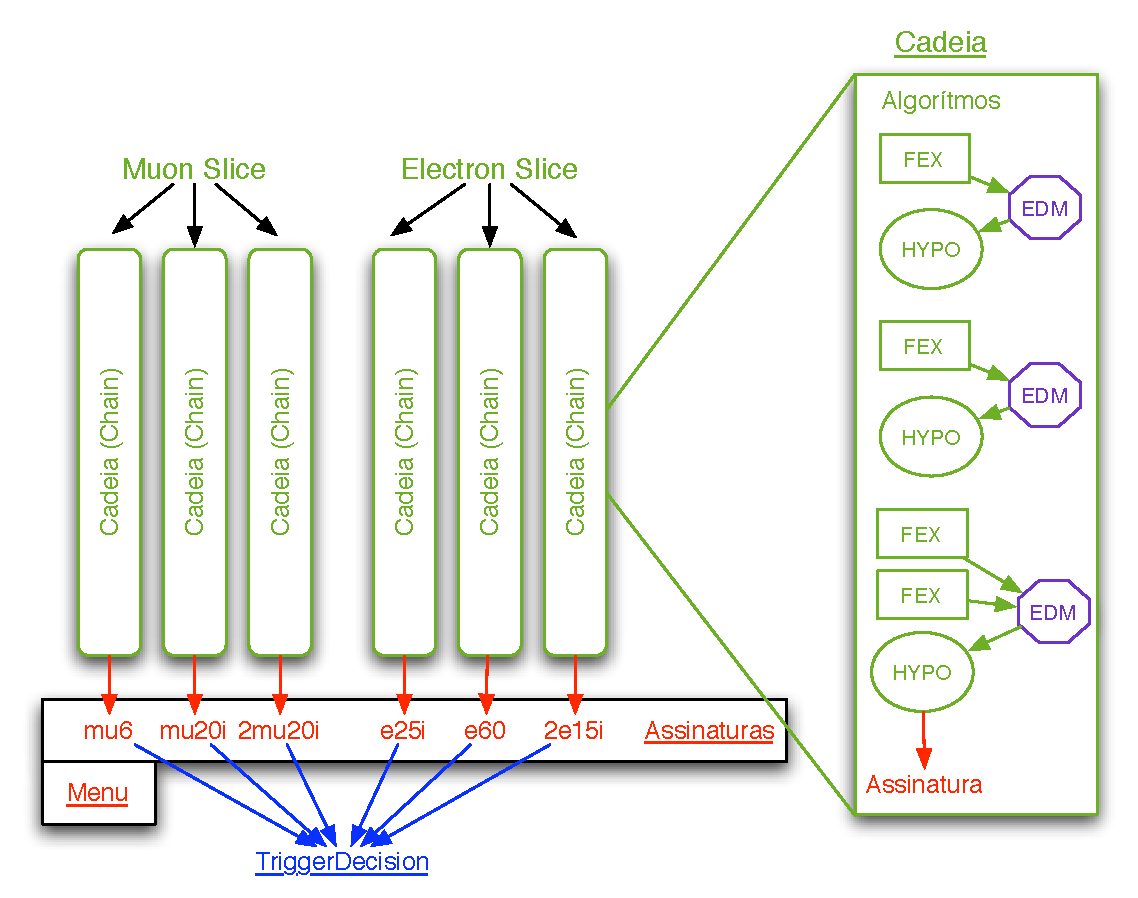
\includegraphics[height = 8cm]{athena_trigger_structure}
\caption{Organização do Athena para a filtragem de alto nível do ATLAS.}
\label{fig:athena_trigger_str}
\end{center}
\end{figure}

Para tornar o desenvolvimento de algoritmos para o sistema de filtragem independente do sistema de fluxo de dados, o Athena implementou camadas de abstração para a comunicação com a L2PU e a PT, de forma que é possível executar os algoritmos \emph{online} em ambiente \emph{offline}, para depois portá-los para o sistema de filtragem do ATLAS.

Durante a execução dos algoritmos de filtragem, é possível salvar em disco o resultado intermediário gerado por cada pacote em um arquivo chamado \emph{NTUPLE}, que pode ser aberto na ferramenta de análise ROOT \cite{bib:site_root} utilizada no CERN. Além disso, a geração de histogramas de qualquer variável de um dado algoritmo é possível, junto com histogramas com as informações de tempo de execução de uma dada parte do código. Tal como as \emph{NTUPLES}, os histogramas também podems er visualizados no ROOT.


\section{Fomatação dos Dados}
\label{sec:eformat}

A informação produzida pelos detectores do ATLAS precisa de uma formatação padronizada, de forma a facilitar a propagação e o processamento da mesma. Este formato deve atender aos seguintes requisitos:

\begin{itemize}

\item Tem que permitir que um evento cresça ou diminua, de acordo com configurações específicas do experimento.

\item Não pode ter uma limitação de tamanho para o evento.

\item Deve ser baseado em fragmentos, onde um fragmento, na sua apresentação mais baixa é o dado de um ROD.

\end{itemize}


Par atender estes requisitos, um formato chamado \emph{EFormat} foi desenvolvido \cite{bib:eformat}. O \emph{EFormat} define a estrutura do dado dentro dos vários estágios do sistema de filtragem de alto nível e do sistema de fluxo de dados. O formato também permite que dados adicionais sejam inseridos, pelo sistema de filtragem, aos dados provenientes do detector, permitindo que porcessos possam identificar rapidamente o tipo e a origem de um evento.

\begin{figure}
\begin{center}
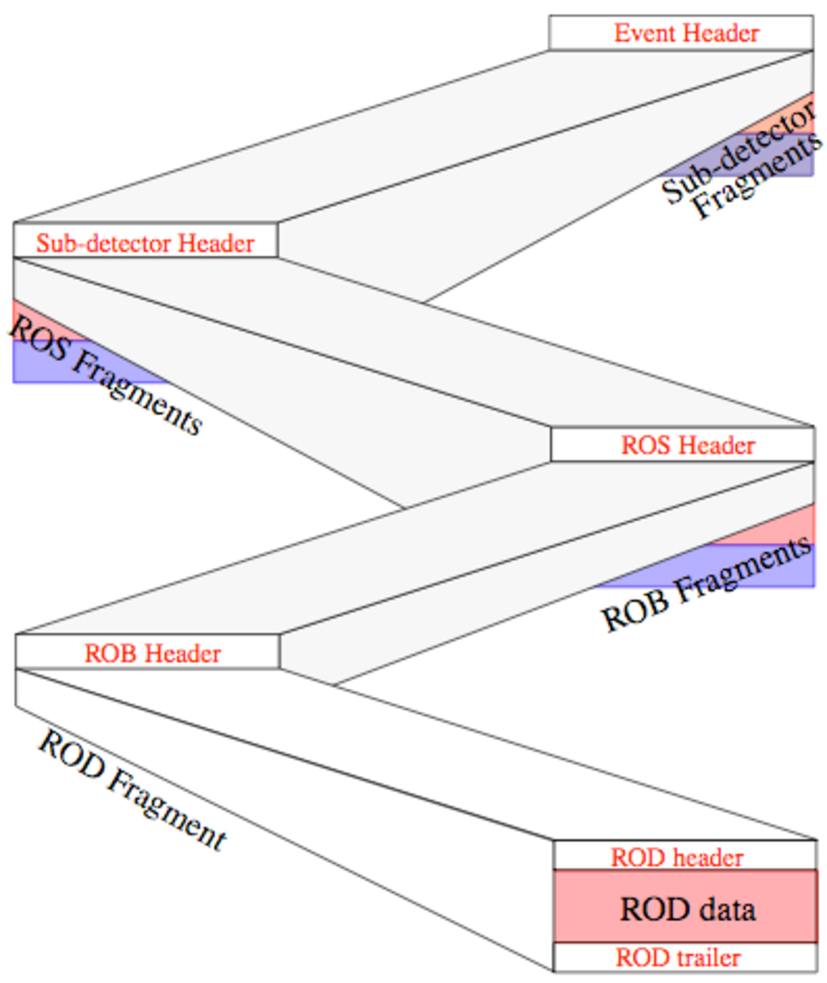
\includegraphics[height = 8cm]{eformat_structure}
\caption{Formato geral dos eventos propagados elo sistema de filtragem de alto nível.}
\label{fig:eformat_structure}
\end{center}
\end{figure}


O formato geral de um evento completo (\emph{Full Event}) pode ser observado na figura~\ref{fig:eformat_structure}. Como se percebe, o evento é composto por fragmentos. Um evento completo é uma união de fragmentos dos subdetectores (calorímetro eletromagnético, detectores de traços, etc), e um fragmento de um dado subdetector é um conjunto de fragmentos de um ROS. Já um fragmento de ROS é um conjunto de fragmentos de ROB. Finalmente, cada fragmento de ROB contém apenas um único fragmento de ROD. Cada fragmento contém um cabeçalho e um rodapé, com informações de identificação do evento (procedência, ideintificação da colisão, etc) e sobre o seu tamanho, para fácil indexação.

Bibliotecas de leitura e escrita para o \emph{EFormat} estão disponíveis para os desenvolvedores do sistema de filtragem de alto nível do ATLAS, de forma a permitir não só a padronização do formato, bem como o seu acesso.

